\section{Public curriculum, verifiable practice and deployment expansion}
\subsection{Delivered scope and assurance boundary}
The current catalog contains 24 skill tracks: the five original technical tracks
and nineteen additional specialisms. Ethical hacking and offensive security map to
foundations, web/pentest and adversary-emulation paths rather than being treated as
unrelated disciplines. New tracks explicitly cover red teaming, SOC analysis, Active
Directory, cloud, containers/Kubernetes, DevSecOps, DFIR, threat intelligence/hunting,
malware analysis, mobile and API security, cryptography, wireless/IoT, OT/ICS,
architecture/GRC, vulnerability management, bug bounty and AI application security.
The catalog is broad rather than an assertion that cybersecurity has a final,
exhaustive taxonomy. Each specialist path has eight main levels, explicit entry
background, changed-case and control assessments, and later reasoning practice.

A separate eight-task verified practice project gives an immediate route through
five generated exercises and three real Juice Shop checks. The home lab is public:
personal completed-history assumptions were removed, host variables are placeholders,
Bandit starts at challenge zero, and legacy IDs remain stable. The defensive path
now starts with generated request logging; demonstrating a real host log source
remains a separate task. Existing completion history is preserved without claiming
it has passed the new verification criteria.

Across all 28 bundled packs, including the two general examples, there are 1,002
expanded task nodes: 348 bundled exercise checks, 42 signed CTF checks, 448 artifact
checks, four command checks and 160 manual tasks. Thus 842 tasks have a non-manual
check, but only 390 require an exact exercise result or signed game observation.
The nineteen new specialist paths each have 18 graded concept/micro-exercise checks
and 16 practical artifact checks. Many of the 348 checks are two-choice reasoning
questions: repeated guesses can pass, so their evidence is weaker than independent
problem solving. Counts must not be presented as 842 verified practical skills.
Narrative explanations, unfamiliar practical variants and professional judgment
still need review. Adding a file-size check cannot resolve that assessment gap.

\subsection{Research and reproducible authoring}
The evidence register now contains 55 inspected sources with access dates, supported
inferences and limitations. Additions use official MITRE emulation plans, Microsoft
SOC/AD/AD CS documentation, OWASP standards and lab projects, Kubernetes guidance,
NIST/CISA/FIRST material, DigitalCorpora, CryptoHack, and relevant platform projects.
The existing learning-research and practitioner review remains the methodological
basis. A 404 HTB red-team path and a 403 ZeroPoint page were not treated as inspected
syllabi. No claim of empirical learning effectiveness or career success is made.

Canonical specialist learning data lives in
\path{docs/curriculum/specialist-paths.json}. The generator emits nineteen packs,
152 authored cases, the specialist assessment crosswalk, export copies and catalog
metadata. The original forty assessments remain in their separate source map. The
LaTeX builder includes all 192 assessments and the source register in the complete
handbook/report. Runtime TOML and JSON remain machine-readable formats; the complete
human documentation is maintained in LaTeX, with selected duplicated Markdown commands.

\subsection{Verified behavior and fixes found during integration}
The full expanded suite passed 141 tests, including browser flows at mobile and
desktop widths. Server tests reject wrong answers, JSON type confusion, manual
completion bypass, cross-account evidence, stale/superseded instances, forged/stale
receipts and duplicate rewards. Browser tests exercise the full logging solve,
verified XP and role search. The timer preserves keyboard focus while updating.

A disposable Docker integration actually launched Juice Shop, WebGoat and MQTT.
It verified login/HTTP reachability, a real MQTT message round trip, container limits,
internal target networks and blocked external TCP egress. A browser changed Juice
Shop's scoreboard challenge from unsolved to solved; a signed observation then
completed only the assigned account's corresponding Ascend task. The unsolved
injection task remained incomplete. The host collector refuses to assign one game
container to two learners and serializes concurrent invocations.

Testing found three deployment defects: internal-only target port publishing was
ineffective on the tested Docker version; WebGoat's upstream curl health probe used
a binary absent from its image; and the tracker build implicitly consumed an AMD64
wheel cache. Fixed TCP gateways, a Java health probe and explicit offline-cache
opt-in address those respective defects. The normal tracker image was built from
its pinned base and dependency constraints. The shipped hardened Compose and proof
overlay were tested with temporary data, including persistence across a restart.
The documented backup/restore procedure was exercised against disposable volumes.
The first restart smoke attempt reused an ephemeral host port; Docker reassigned it.
The test now resolves the port after restart, and the retained final run passed.

Five pinned image indexes provide both AMD64 and ARM64. The complete pinned dependency
set resolves to 36 compatible CPython 3.12 ARM64 wheel artifacts; http-ece is built
as a pure-Python universal wheel from its pinned source. No x86 wheel was reused for
ARM. Bandit authentication uses a private short-lived control connection because
restricted level shells do not uniformly accept an identity command. These checks do not establish physical Raspberry Pi boot, thermal behavior,
RAM demand under load or ARM runtime correctness. The Pi acceptance step remains
running the documented smoke tests on the user's 64-bit OS, one optional lab at a time.
Live Bandit authentication and live notification-provider delivery were not performed.

\subsection{Local installation and retained evidence}
A fresh private backup preceded the local pack update. The six existing private
packs matched the recorded baseline, so there were no private curriculum edits to
merge. All supplied packs were installed while preserving the active defensive
mission and every existing entry and node state. Database integrity was checked;
no test completions or XP were added to the real profile. A first restart followed
the virtualenv Python symlink to the system interpreter and lacked FastAPI; launching
via the virtualenv path corrected it. HTTP health and the new logging next task were
then checked against the local server.

The public distribution is \path{tracks/cyber-tracks-v4.zip}, containing 26 packs
(the 24 skill tracks plus home lab and verified practice), seven PDFs and LaTeX
sources. Rebuild it with \texttt{python3 scripts/package\_tracks.py} after building
the documents. It requires the current Ascend backend; copying packs alone does not
upgrade an older verifier engine.

CI also checks specialist generation consistency. Home-lab upgrade regression uses
a preserved v3 fixture, so it works in a shallow checkout without old Git objects.

Feature-sized commits and their recorded validation appear in the status table.
Detailed transcripts are retained under \path{docs/testing/}, including
\path{verified-learning.txt}, \path{expanded-release.txt}, \path{docker-labs.txt},
\path{deployment-integration-final.txt}, \path{restore-smoke.txt},
\path{arm64-compatibility.json} and \path{expanded-install.txt}.

\begin{figure}[htbp]
\centering
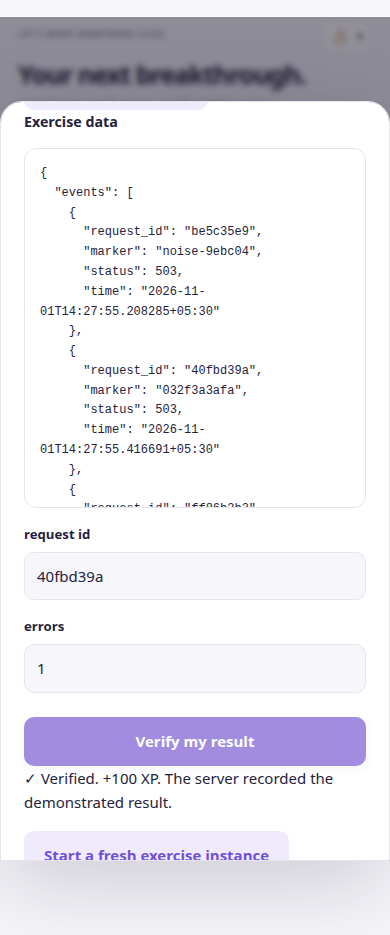
\includegraphics[width=.38\textwidth]{verified-lab-390.png}
\caption{Mobile browser integration: a generated logging result passes server verification. All displayed evidence and XP belong to a disposable test profile.}
\end{figure}
